\documentclass[11pt]{article}
\usepackage[a4paper,margin=1in]{geometry}
\usepackage[T1]{fontenc}
\usepackage{lmodern}
\usepackage{microtype}
\usepackage{amsmath,amssymb,amsthm,mathtools}
\usepackage{booktabs,array,enumitem,graphicx,longtable,xcolor}
\usepackage[numbers,sort&compress]{natbib}
\usepackage[colorlinks=true,linkcolor=blue!55!black,citecolor=blue!55!black,urlcolor=blue!55!black]{hyperref}

\newtheorem{theorem}{Theorem}[section]
\newtheorem{proposition}[theorem]{Proposition}
\newtheorem{corollary}[theorem]{Corollary}
\theoremstyle{definition}
\newtheorem{definition}[theorem]{Definition}
\theoremstyle{remark}
\newtheorem{remark}[theorem]{Remark}
\newcommand{\cD}{\mathcal D}
\newcommand{\cH}{\mathcal H}
\newcommand{\cT}{\mathcal T}
\newcommand{\cW}{\mathcal W}
\newcommand{\spec}{\operatorname{spec}}
\newcommand{\Tr}{\operatorname{Tr}}

\title{\textbf{Prime Dynamics Program, Volume I}\\
\Large Foundations and a Conditional Hilbert--Polya Architecture\\
\large RH-1--RH-160, Five Bold Interfaces, and a Conditional Spectral-Divisor Closure Theorem}
\author{Liang Wang}
\date{July 2026}

\begin{document}
\maketitle

\begin{abstract}
This first volume of a four-volume synthesis compresses one hundred and sixty
RH-numbered papers that developed the prime-dynamics
program from its original symbolic analogy into a collection of exact
theorems, validated finite models, conditional all-level compositions, and
sharp negative results.  The volume of local work now obscures the global
question: what is the shortest honest chain from the existing dynamical
foundation to a Hilbert--Polya conclusion?

We give a deliberately bold minimum viable proof architecture.  Its rigorous
foundation $F$ consists of the corrected sieve--kneading coordinate,
parity-resolved deterministic trace geometry, the fixed-noise intrinsic
regularized determinant, continuum bridges, and finite certification
technology.  Five additional interfaces are stated as hypotheses, not
results: $A$, a canonical all-level pole-renormalized determinant; $B$, an
order-sensitive canonical scattering completion; $C$, a self-adjoint
generator with an intrinsic Riemann--von Mangoldt counting law; $D$, a
target-independent prime-power trace formula with von Mangoldt weights; and
$E$, a no-missing/no-spurious spectral-divisor completeness theorem.

The analytic closure step is elementary but decisive.  Write
$\Xi(z)=\xi(\tfrac12+iz)$.  If the self-adjoint determinant $D_H$ produced by
$A$--$C$ and the arithmetic identity $D$--$E$ give
\[
  \frac{D_H'(z)}{D_H(z)}=\frac{\Xi'(z)}{\Xi(z)}
\]
on one nonempty pole-free domain, with one normalization value, then analytic
continuation gives $D_H=\Xi$.  Since zeros of a self-adjoint spectral
determinant are real, every nontrivial zeta zero lies on the critical line.
This is a conditional implication, not a proof that any of $A$--$E$ holds.

An automated audit finds RH-1 through RH-160 exactly once, each with source
and a PDF; 131 machine-readable verification archives expose 1,717 declared
publication hashes, all of which match.  It also records nine shortcuts
already ruled out by the program.  The unique architecture-relative proof
debt is $\{A,B,C,D,E\}$; the immediate frontier is still $A$.  The result is
therefore a compact, falsifiable research contract for subsequent careful
papers, not an unconditional Stage A, Hilbert--Polya operator, zeta identity,
or proof of the Riemann Hypothesis.
\end{abstract}

\noindent\textbf{Keywords:} Hilbert--Polya program; transfer operator;
regularized determinant; scattering; explicit formula; research roadmap;
validated numerics.

\section{The four-volume series and the boundary of Volume I}

The numbered corpus remains the atomic source of mathematical claims.  The
four synthesis volumes reorganize those sources by function; they do not
concatenate proofs, change theorem status, or create a new numbered result.
The partition is
\begin{center}
\begin{tabular}{clp{8.3cm}}
\toprule
volume & source range & role\\
\midrule
I & RH-1--RH-160 & symbolic and fixed-noise foundations, finite certification,
reset architecture, and the conditional interfaces A--E\\
II & RH-161--RH-241 & packet-to-Riesz assembly, temporal clouds, relative
determinants, and the moving trace-envelope frontier\\
III & RH-242--RH-281 & deterministic numerator anchors, selectors, analytic
tails, and counterloops\\
IV & RH-282--RH-361 & noisy heads, annular endpoints, first alias, and signed
completion\\
\bottomrule
\end{tabular}
\end{center}

Volume I stops at RH-160.  RH-161 is an independent typed assembly theorem
and is the first source of Volume II.  Later volumes may sharpen the location
of the active frontier, but they do not retroactively prove any of the five
interfaces formulated here.  In particular, the series organization carries
no Gate A--E promotion.

\section{Purpose: replace 160 local layers by one research contract}

The original project began with a numerical and symbolic correspondence
between cumulative sieve words and a quadratic map.  RH-1 made the first
essential correction: ordered convergence to a kneading coordinate is
unconditional, whereas universal finite-stage admissibility is false and
equality of one itinerary does not imply topological conjugacy
\citep{WangRH1,WangPublished}.  The subsequent sequence did not repair the
old word ``isomorphism'' by rhetoric.  It changed the object.

The durable spectral object is a nonselfadjoint, parity-renormalized transfer
determinant.  At fixed positive noise it is intrinsic and has rigorous
continuum limits; its deterministic small-noise geometry contains genuine
bulk poles.  The noisy Markov operator itself is irreversible and cannot be
declared to be a Hilbert--Polya operator \citep{WangRH7,WangRH45}.  Later
papers developed directional Hardy/Stein bounds, packet reductions,
outward-rounded certificates, correlated support cocycles, and spectral
resets \citep{WangRH50,WangRH100,WangRH149,WangRH160}.

This paper intentionally changes altitude.  It does not add a finer packet
estimate.  Instead it asks for the smallest chain of mathematical interfaces
which, if proved in later papers, would turn the existing foundation into a
complete spectral realization.  ``MVP'' means \emph{minimum viable proof},
not minimum numerical resemblance.

Three rules govern the synthesis.
\begin{enumerate}[label=\textbf{R\arabic*.},leftmargin=3.2em]
\item A finite certificate never becomes an eventual theorem by repetition.
\item A conditional composition never proves its physical hypotheses.
\item No zero ordinate, fitted map to height, or target spectral list may be
inserted into the construction that is supposed to explain that list.
\end{enumerate}

Throughout, \emph{proved} means an analytic theorem in its stated scope,
\emph{certified} means a finite outward or exact-stored computation,
\emph{conditional} means a valid implication whose physical hypotheses are
still open, and \emph{open} means that even the required implication has not
yet been constructed.  A no-go result rejects only the route named in its
statement.  These labels are not interchangeable, and the audit never
promotes one by numerical repetition.

\section{What the 160 layers actually established}

Table~\ref{tab:phases} compresses the sequence by mathematical function.
The endpoints are not equal in logical strength: an analytic theorem, an
exact stored-matrix certificate, floating evidence, a conditional theorem,
and a no-go are different output types.

\begin{table}[t]
\centering
\small
\renewcommand{\arraystretch}{1.13}
\begin{tabular}{c>{\raggedright\arraybackslash}p{4.0cm}>{\raggedright\arraybackslash}p{7.8cm}}
\toprule
layers & phase & durable conclusion and boundary\\
\midrule
1--3 & symbolic foundation & ordered sieve--kneading convergence, inverse
prime realization, and parity geometry; no natural topological conjugacy\\
4--15 & determinant hygiene & continuum response, irreversible $\det_2$,
ordered traces, deterministic flat traces, postcritical zeta factors, and
genuine bulk poles; no self-adjoint interpretation\\
16--45 & packet, Feshbach, validation & critical-branch packets, complete
finite contour certificates, dyadic continuum bridges, and fixed-noise
intrinsic determinant convergence; no zero-noise determinant theorem\\
46--71 & small-noise directional control & pole obstruction, directional
Hardy--Stein reduction, phase-aware finite horizons, and a closed frozen
production chain; family-uniform all-level control remains open\\
72--100 & Stage-A alternatives & validated assembly, effective-rank and Schur
packet corridors, moving-cloud relative determinant target, and an audited
completion frontier; Stage A and A5 remain unproved\\
101--129 & exterior support and recurrence & finite memory actions,
fourth-cross/exterior support, adaptive certificates, and sharp conditional
eventual-support theorems; physical all-level recurrence is absent\\
130--149 & gauge, viability, source closure & floor-free semidefinite theory,
moving-frame tail recurrences, outward finite composition, source enclosures,
and an inclusion-minimal three-interface conditional route\\
150--160 & reset dichotomy & independent spectral resets, coherent
transitions, a finite native support floor, exact contemporaneous-cross
cancellation, complete lag-$\leq8$ finite cross closure, and a conditional
all-level native/directional theorem\\
\bottomrule
\end{tabular}
\caption{A functional compression of RH-1--RH-160.}
\label{tab:phases}
\end{table}

The strongest current all-level statement is RH-160's implication.  Eventual
overlap conditioning, weak-eigenvalue/tail separation, and selected spectral
spread imply a uniform native floor; adding a bounded-lag fourth-cross law
gives a directional seed.  Every clause passes on the five frozen scales,
but no clause is proved eventually.  The gap between ``120/120'' and
``all sufficiently large levels'' is precisely the first macro interface
below.

\subsection{Negative knowledge is part of the result}

The sequence has closed several attractive shortcuts.  They must not reappear
inside an optimistic roadmap under new names:
\begin{enumerate}[leftmargin=2.1em]
\item one shared kneading word does not give topological conjugacy (RH-1);
\item the irreversible noisy Markov operator is not directly self-adjoint
under a positive stationary weight (RH-7);
\item $AB$ and $BA$ spectra do not record temporal orientation (RH-8);
\item a plain entire small-noise determinant cannot cross the genuine
deterministic poles without renormalization (RH-15, RH-46);
\item noise-uniform fixed-step global complement contraction is impossible
(RH-50);
\item finite-anchor regression cannot prove an eventual scale law (RH-117);
\item independent interval balls can destroy positivity retained by a
correlated congruence (RH-153);
\item a contemporaneous full-memory spectral reset sees only negative tail
coupling in its recent cross action (RH-157);
\item inverse prime encoding is not a target-independent von Mangoldt trace
formula (RH-1--2).
\end{enumerate}

These no-go results do not weaken the MVP.  They make its interfaces narrow
enough to be meaningful.

\section{The minimum viable objects}

Let
\[
 \xi(s)=\frac12s(s-1)\pi^{-s/2}\Gamma(s/2)\zeta(s),
 \qquad \Xi(z)=\xi\!\left(\frac12+iz\right).
\]
The function $\Xi$ is entire and even, and the Riemann Hypothesis is
equivalent to all its zeros being real \citep{Titchmarsh1986}.  This notation
is used only to state the target and to verify the final identity; $\Xi$ and
its zero set are forbidden inputs to interfaces $A$--$D$.

The existing finite/noisy family will be denoted schematically by
$K_{n,\sigma}$, after Perron/parity removal and the time-ordering required by
the quadratic dynamics.  Its exact implementation may evolve.  The MVP
requires only that each interface produce a canonical output for the next.
Regularized determinant statements use the standard trace-ideal convention
\citep{Simon2005}; a canonical-system realization is one possible, but not
presupposed, implementation of the self-adjoint gate \citep{deBranges1968}.

\begin{definition}[Foundation $F$]
$F$ is the conjunction of results already proved in their stated scopes:
the corrected symbolic coordinate and parity factor, intrinsic fixed-noise
regularized traces/determinants, deterministic pole structure, continuum and
finite-section bridges, and the finite certification toolkit.  It does not
include an eventual small-noise theorem.
\end{definition}

The foundation is useful even if every later interface fails.  It supports a
standalone theory of nonselfadjoint transfer spectra.

\section{Five bold interfaces}

The following are deliberately stronger than the presently proved results.
They are hypotheses with exact success and failure tests.

\subsection{\texorpdfstring{$A$}{A}: canonical all-level intrinsic determinant}

There exist an admissible joint schedule $(n,\sigma)\to(\infty,0)$, an exact
moving-cloud factor $C_{n,\sigma}$, and a zero-free normalization
$Z_{n,\sigma}$ such
that
\[
 \cD_{n,\sigma}(z)
 =Z_{n,\sigma}(z)
   \frac{\det{}_2\!\bigl(I-zK_{n,\sigma}^{\rm bulk}\bigr)}
        {C_{n,\sigma}(z)}
 \longrightarrow \cD_{\rm dyn}(z)
\]
locally uniformly on compacta after removable cloud zeros have been filled
by the exact reducing factorization.  Together with the explicitly tracked
deterministic pole divisor, this defines the canonical meromorphic dynamical
object.  The residual limit is not identically zero, is independent of all
admissible meshes, packet gauges, reset choices, and cutoffs, and preserves
the required directed three/six-step trace data.  The use of the actual cloud
factor is forced by RH-80's fixed-factor no-go and exact relative determinant
algebra \citep{WangRH80}.

RH-160 suggests two possible internal realizations: a minimal native-reset
route using the O/E/S interfaces, or a directional route adding bounded lag
L.  Both still require a typed all-level assembly.  Gate $A$ fails if any
required running margin tends to zero along an infinite scale sequence, if
the normalization is target dependent, or if different admissible schedules
give inequivalent limits.

\subsection{\texorpdfstring{$B$}{B}: canonical order-sensitive scattering completion}

The dynamical limit admits a unique, functorial completion to an inner or
unitary scattering object $S_{\rm dyn}(z)$.  Its determinant is related to
$\cD_{\rm dyn}$ by a proved factorization, its boundary values are unitary on
a real axis, and its lifted phase retains a nonzero directed temporal trace.
It is independent of arbitrary dilations and auxiliary channels.

A generic unitary dilation is insufficient: infinitely many dilations can
share one compression while carrying arbitrary extra spectrum.  Gate $B$
fails if all canonical completions erase temporal orientation or if
uniqueness requires a fitted branch choice.

\subsection{\texorpdfstring{$C$}{C}: self-adjoint generator and intrinsic counting}

There is a canonical self-adjoint operator $H$ (or canonical system) whose
scattering/regularized determinant $D_H$ is the completed object from $B$.
Its domain, self-adjointness, spectral multiplicities, and completeness are
proved.  With multiplicity, set
\[
 N_H(T)=\#\{\lambda\in\operatorname{spec}_{\rm disc}(H):0<\lambda\leq T\}.
\]
Before using zeta ordinates, one derives from $H$ itself
\[
 N_H(T)=\frac{T}{2\pi}\log\frac{T}{2\pi}
        -\frac{T}{2\pi}+O(\log T).
\]
The precise lower-order form may be reached in stages, but the leading
$T\log T$ law cannot be manufactured by fitting $T=T(\sigma)$.  Gate $C$
fails if the only canonical object has bounded phase, logarithmic-only rank,
a power-law Weyl exponent, uncontrolled extra spectrum, or wrong
multiplicity.

\subsection{\texorpdfstring{$D$}{D}: target-independent prime-power trace formula}

For a separating test class $\cT$ for which $h(H)$ is trace class, use the
Fourier convention
\[
 h(t)=\int_{\mathbb R}g(u)e^{itu}\,du.
\]
The trace of $H$ is derived from the dynamics/arithmetic interface in the
form
\[
 \Tr h(H)
 =\cW_\infty(h)
 -\sum_{m\ge2}\frac{\Lambda(m)}{\sqrt m}
   \bigl(g(\log m)+g(-\log m)\bigr),
 \qquad h\leftrightarrow g.
\]
Here $\cW_\infty$ contains the exactly matched archimedean, pole, and
normalization terms.  Prime powers and von Mangoldt weights must emerge from
a proved transform; no zeta-zero data are permitted.  The parallel TPC
program may supply arithmetic lemmas only after a theorem matches variables,
test functions, weights, and counterterms.  A common use of the word
``trace'' is not an interface.

Gate $D$ fails if the weights have to be inserted by hand, if only primes but
not prime powers occur, if the test class is too small to determine a
divisor, or if a target-informed inverse parameter supplies the answer.

\subsection{\texorpdfstring{$E$}{E}: spectral-divisor completeness}

The trace identity from $D$, together with the classical explicit formula,
is upgraded to an identity of meromorphic logarithmic derivatives on one
nonempty common domain:
\[
 \frac{D_H'}{D_H}=\frac{\Xi'}{\Xi}.
\]
Every sector of $H$, every gamma/pole term, and every finite normalization is
accounted for.  A single reference value fixes the zero-free constant.  Gate
$E$ fails upon any missing or spurious level, hidden entire factor,
multiplicity mismatch, or unmatched archimedean term.

Unlike a claim that ``the spectra look alike'', $E$ is a complete identity
with a yes/no verification target.  It is deliberately close to the final
target and is expected to carry major proof debt; listing it as an interface
does not make it plausible or inexpensive.

The arrows $A\to B\to C\to D\to E$ describe functional dependencies, not a
license to hide target information upstream.  Gates $A$--$D$ may use the
sieve, the quadratic dynamics, and previously proved analytic constructions,
but not values of $\Xi$ or its zeros.  Gate $E$ is the first comparison with
the completed zeta function.  Finite prototypes of later gates may be run
early as falsification tests, but they do not alter this proof order.

\section{The conditional closure theorem}

The difficult work lies in proving $A$--$E$.  Once they are available, the
last analytic implication is short and rigorous.

\begin{theorem}[Spectral-divisor closure]\label{thm:closure}
Let $H$ be self-adjoint and suppose it has an entire regularized spectral
determinant $D_H$ whose zero divisor, with multiplicity, is exactly the
discrete spectrum of $H$.  Let $U\subset\mathbb C$ be a nonempty connected
open set on which $D_H$ and $\Xi$ are nonzero.  If
\[
 \frac{D_H'(z)}{D_H(z)}=\frac{\Xi'(z)}{\Xi(z)}
 \qquad(z\in U)
\]
and $D_H(z_0)=\Xi(z_0)$ at one $z_0\in U$, then
\[
 D_H(z)=\Xi(z)\qquad(z\in\mathbb C).
\]
Consequently every nontrivial zero of $\zeta$ lies on the critical line.
\end{theorem}
\begin{proof}
On $U$, the quotient $Q=D_H/\Xi$ obeys $Q'/Q=0$, so it is constant.
The normalization gives $Q=1$ on $U$.  Hence the entire function
$D_H-\Xi$ vanishes on a nonempty open set.  The identity theorem gives
$D_H=\Xi$ on all of $\mathbb C$.

All zeros of a spectral determinant whose divisor is the spectrum of a
self-adjoint operator are real.  If $\Xi(z)=0$, then
$\rho=\tfrac12+iz$ is a nontrivial zeta zero; real $z$ gives
$\operatorname{Re}\rho=\tfrac12$.
\end{proof}

\begin{corollary}[Conditional MVP implication]\label{cor:mvp}
Assume foundation $F$ and prove interfaces $A$--$E$ with the compatibility
specified above.  Then the construction satisfies the hypotheses of
Theorem~\ref{thm:closure}, and the Riemann Hypothesis follows.
\end{corollary}
\begin{proof}
$A$ supplies the canonical dynamical determinant, $B$ its canonical
order-sensitive completion, and $C$ the self-adjoint determinant $D_H$.
$D$ supplies the zero-free arithmetic trace identity without using zeros as
input.  $E$ proves completeness, upgrades that identity to the logarithmic
derivative equality, and fixes normalization.  Apply
Theorem~\ref{thm:closure}.
\end{proof}

\begin{remark}[What the corollary does not say]
Corollary~\ref{cor:mvp} is not evidence for any premise.  In particular,
assuming $E$ casually would merely assume the hardest spectral identity.
Its value is architectural: every later paper can be judged by whether it
proves a named part of $A$--$E$, finds a counterexample, or leaves the debt
unchanged.
\end{remark}

\section{Minimal proof debt and route alternatives}

Treat the MVP as the monotone dependency formula
\[
 \mathrm{MVP}=F\wedge A\wedge B\wedge C\wedge D\wedge E.
\]
A proved leaf contributes no debt; a finite or conditional leaf contributes
its name; a no-go leaf kills its branch.  AND takes unions and OR takes the
inclusion-minimal antichain of alternatives.  This elementary recursion was
used in earlier route reviews and is re-audited here.

\begin{proposition}[Architecture-relative completion frontier]
With the statuses established after RH-160, the unique inclusion-minimal
completion bundle for the full MVP is
\[
 \boxed{\{A,B,C,D,E\}}.
\]
The bundle required to reach a genuine Hilbert--Polya \emph{candidate}, prior
to arithmetic identification, is $\{A,B,C\}$.  The current first missing
gate is $A$.
\end{proposition}
\begin{proof}
$F$ is closed in its stated scope.  The reset-support subroute inside $A$ has
a conditional theorem and finite evidence, but its typed determinant
assembly is absent, so $A$ itself is open.  Gates $B$--$E$ are also open.  The
formula is a conjunction, so
every nonclosed leaf is required.  Removing $D$ or $E$ leaves a
self-adjoint but non-arithmetic model; removing $C$ leaves no real spectral
axis; removing $B$ leaves no canonical completion; removing $A$ leaves no
all-level dynamical object.
\end{proof}

This minimality is relative to the present architecture.  A future theorem
may prove two interfaces simultaneously.  It may not silently omit their
mathematical functions.

Inside $A$ there are two typed alternatives:
\[
 A_{\rm native}\quad\text{or}\quad A_{\rm lagged}.
\]
The native route assumes less and should be tried first if downstream
assembly accepts compression support.  If four directional images are
essential, RH-159 proves that native positivity cannot replace them, and the
adaptive-lag route is required.  Failure of lagged cross support therefore
does not automatically kill the native route.

\begin{figure}[t]
\centering
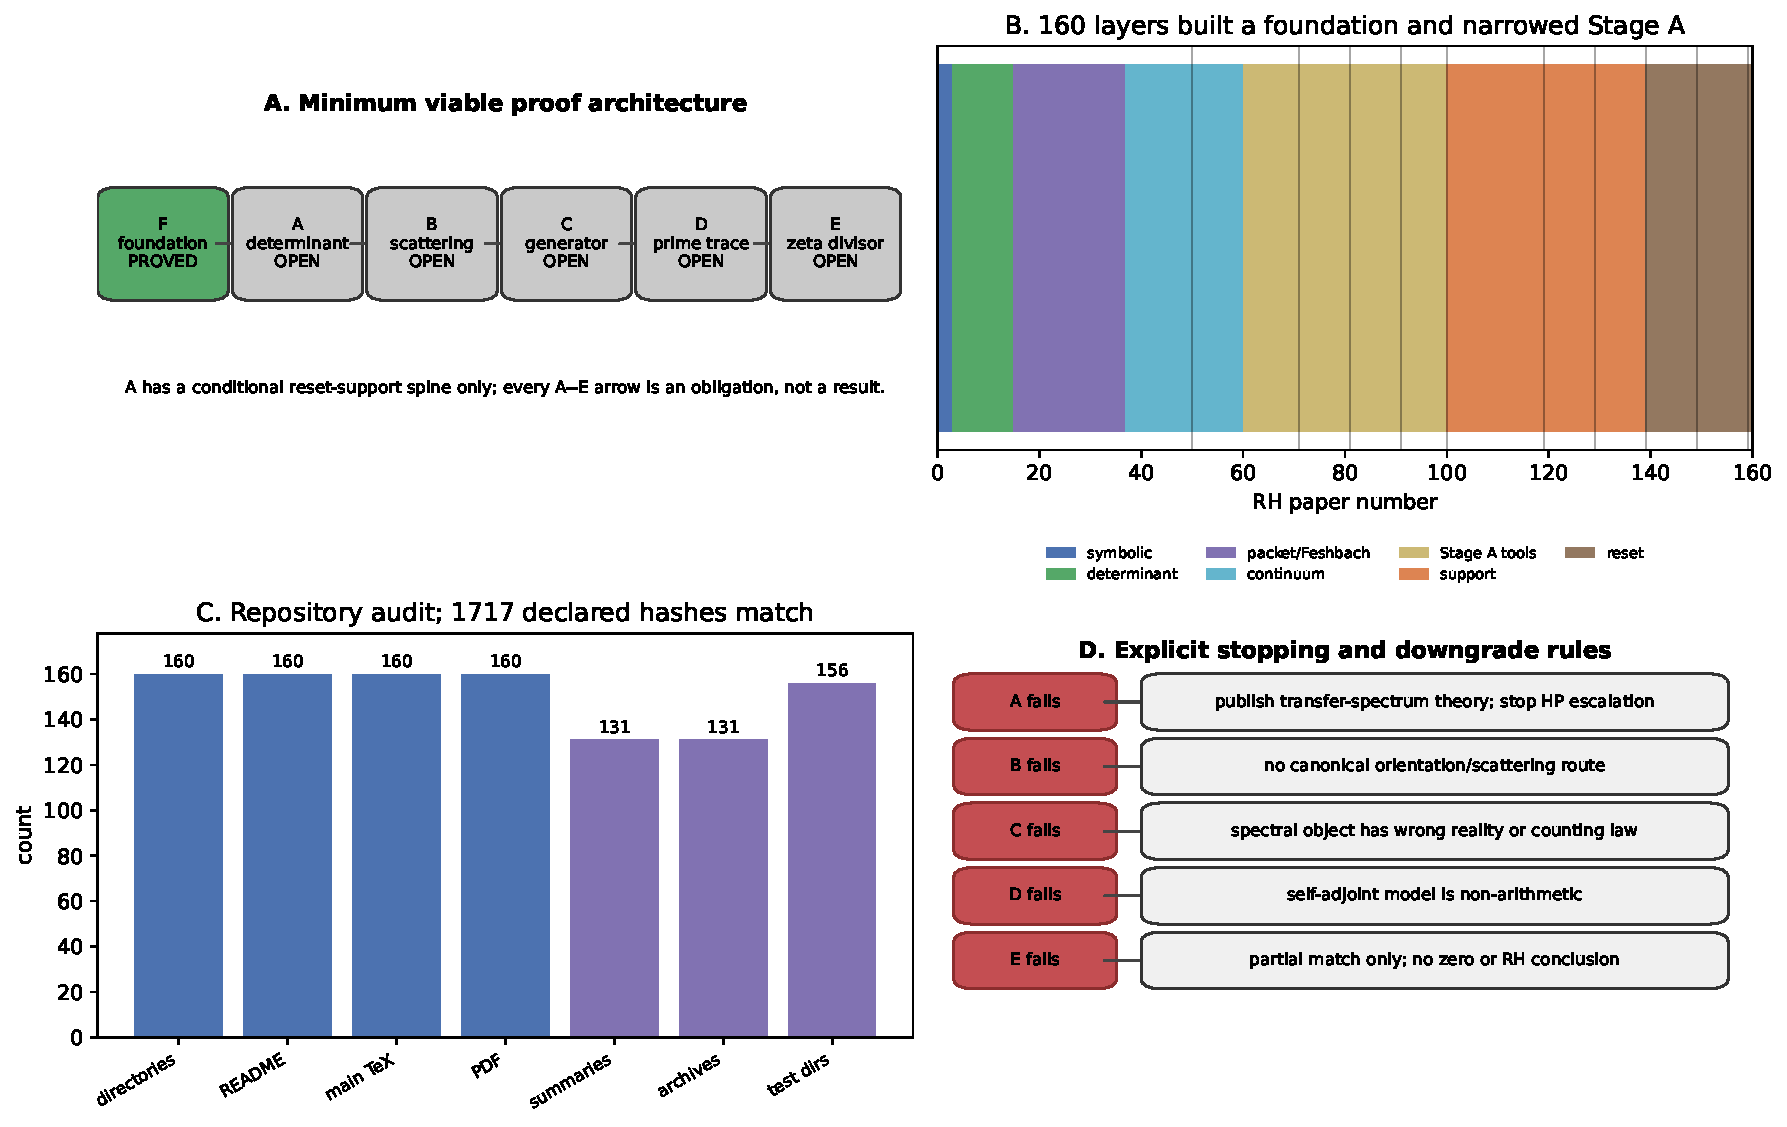
\includegraphics[width=\textwidth]{figures/conditional_mvp_roadmap.pdf}
\caption{The minimum viable architecture, the 160-layer phase ledger,
repository audit, and explicit downgrade rules.}
\label{fig:roadmap}
\end{figure}

\section{A coarse but complete execution plan}

The purpose of the MVP is to license bold exploration while keeping later
verification local.  The recommended sequence is:

\begin{enumerate}[label=\textbf{MVP-\arabic*.},leftmargin=4.2em]
\item \textbf{Close or kill $A$.}  Prove one eventual reset route and a typed
all-level moving-cloud quotient assembly.  The native O/E/S route is primary;
bounded lag L is activated only if the assembly needs directional cross rank.
\item \textbf{Prototype $B$ before polishing $A$ constants.}  On the best
finite models, search for a normalization-unique inner/scattering completion
and test whether the RH-8 directed trace survives.  A rigorous no-go here can
save many all-level estimates.
\item \textbf{Demand $C$ without ordinate fitting.}  Construct the candidate
self-adjoint domain and derive its counting law from phase or geometry.  If
the leading law is not $T\log T$, stop the Hilbert--Polya escalation.
\item \textbf{Build $D$ as an arithmetic transducer.}  Start from primitive
dynamical traces and derive prime powers, von Mangoldt weights, and
archimedean terms on one test class.  Use TPC machinery only through an exact
crosswalk theorem.
\item \textbf{Prove $E$ last.}  Compare logarithmic derivatives, close hidden
sectors and zero-free factors, verify multiplicities, and invoke
Theorem~\ref{thm:closure} only after all inputs are independent of zero data.
\end{enumerate}

The ordering is intentionally not ``finish every estimate before asking if
the next object exists''.  Cheap finite prototypes of $B$ and $C$ are useful
falsification experiments.  They do not promote those gates to theorems.

\section{Stopping rules and publishable downgrade outcomes}

Each macro gate has a clean negative outcome.

\begin{table}[ht]
\centering
\small
\renewcommand{\arraystretch}{1.12}
\begin{tabular}{c>{\raggedright\arraybackslash}p{5.4cm}>{\raggedright\arraybackslash}p{6.4cm}}
\toprule
gate & decisive failure & honest surviving result\\
\midrule
$A$ & all admissible all-level routes lose overlap, tail separation, spread,
or schedule independence & rigorous nonselfadjoint fixed-noise and finite
small-noise transfer-spectrum theory\\
$B$ & every canonical completion is orientation-blind or nonunique & a
renormalized dynamical determinant with no Hilbert--Polya escalation\\
$C$ & no self-adjoint realization, or intrinsic counting differs from
$T\log T$ & canonical scattering theory with the wrong spectral universality\\
$D$ & no target-independent von Mangoldt/prime-power transform & a
self-adjoint dynamical model that is spectral but not arithmetic\\
$E$ & missing/spurious levels, hidden factors, or multiplicity mismatch & a
partial explicit-formula correspondence with no zero-location conclusion\\
\bottomrule
\end{tabular}
\caption{Failure does not erase earlier mathematics; it fixes the correct
publication level.}
\label{tab:stopping}
\end{table}

These rules are especially important for $C$--$E$.  Numerical agreement of
the first ordinates cannot compensate for a wrong counting law.  A correct
counting law cannot compensate for absent prime-power weights.  A
prime-weight resemblance cannot compensate for missing gamma terms or hidden
spectrum.

\section{Repository audit and reproducibility}

The automated audit discovers RH-1 through RH-160 by directory name rather
than by a hand-written count.  Every integer occurs exactly once.  All 160
directories contain a README, a main TeX source, and at least one PDF; 131
contain machine-readable summaries and verification archives, and 156 have
test directories.  Replaying every declared publication hash in those 131
archives gives 1,717 matches and zero failures.  Seventeen milestone inputs
from RH-1, each decadal layer through RH-60, and the later route reviews are
hashed into the present audit.

This verifies the recorded corpus, not every theorem in 160 papers.  The
classification still relies on the stated theorem boundaries in the source
papers.  It does, however, make accidental omission, duplicate numbering,
archive drift, and silent promotion of macro gates machine-detectable.

\section{Claim boundary}

RH-MVP1 proves two things: the spectral-divisor closure theorem and a
status-aware synthesis of the existing program.  It then makes five bold,
separately falsifiable assumptions to show what a complete route would look
like.

It does \emph{not} prove the eventual reset interfaces, a joint small-noise
determinant, a canonical scattering completion, a self-adjoint generator, a
$T\log T$ counting law, a von Mangoldt trace formula, a completed-zeta
determinant identity, or the Riemann Hypothesis.  The current unconditional
claim level remains the rigorous dynamical/fixed-noise spectral foundation.

The optimistic conclusion is nevertheless concrete.  The maze no longer
needs 160 simultaneous labels.  It has five doors:
\[
 \boxed{A\longrightarrow B\longrightarrow C\longrightarrow D\longrightarrow E.}
\]
Later papers may carefully prove them, replace one with a genuinely stronger
construction, or close the route by a no-go.  Until then, the diagram is a
research contract, not a theorem about zeta zeros.

\appendix
\section{Atomic source index}

The following machine-generated index lists every canonical numbered source
in Volume I.  It is a provenance locator, not a claim that all entries have
the same theorem status.

\begin{longtable}{r >{\raggedright\arraybackslash}p{0.78\textwidth}}
\toprule
source & canonical directory\\
\midrule
\endfirsthead
\toprule
source & canonical directory\\
\midrule
\endhead
RH-1 & \texttt{RH-\allowbreak{}1-\allowbreak{}rigorous-\allowbreak{}sieve-\allowbreak{}kneading-\allowbreak{}reformulation}\\
RH-2 & \texttt{RH-\allowbreak{}2-\allowbreak{}exact-\allowbreak{}prime-\allowbreak{}kneading-\allowbreak{}spectral-\allowbreak{}stability}\\
RH-3 & \texttt{RH-\allowbreak{}3-\allowbreak{}parity-\allowbreak{}resolved-\allowbreak{}band-\allowbreak{}merging-\allowbreak{}spectrum}\\
RH-4 & \texttt{RH-\allowbreak{}4-\allowbreak{}spectral-\allowbreak{}obstructions-\allowbreak{}renormalized-\allowbreak{}limits}\\
RH-5 & \texttt{RH-\allowbreak{}5-\allowbreak{}renormalized-\allowbreak{}gaussian-\allowbreak{}response}\\
RH-6 & \texttt{RH-\allowbreak{}6-\allowbreak{}continuum-\allowbreak{}spectral-\allowbreak{}double-\allowbreak{}limits}\\
RH-7 & \texttt{RH-\allowbreak{}7-\allowbreak{}irreversible-\allowbreak{}gaussian-\allowbreak{}cycle-\allowbreak{}spectrum}\\
RH-8 & \texttt{RH-\allowbreak{}8-\allowbreak{}time-\allowbreak{}ordered-\allowbreak{}cycle-\allowbreak{}curvature}\\
RH-9 & \texttt{RH-\allowbreak{}9-\allowbreak{}small-\allowbreak{}noise-\allowbreak{}cycle-\allowbreak{}localization}\\
RH-10 & \texttt{RH-\allowbreak{}10-\allowbreak{}parity-\allowbreak{}renormalized-\allowbreak{}long-\allowbreak{}cycle-\allowbreak{}determinant}\\
RH-11 & \texttt{RH-\allowbreak{}11-\allowbreak{}collet-\allowbreak{}eckmann-\allowbreak{}flat-\allowbreak{}trace-\allowbreak{}completion}\\
RH-12 & \texttt{RH-\allowbreak{}12-\allowbreak{}postcritical-\allowbreak{}weighted-\allowbreak{}zeta-\allowbreak{}factorization}\\
RH-13 & \texttt{RH-\allowbreak{}13-\allowbreak{}validated-\allowbreak{}reduced-\allowbreak{}sector-\allowbreak{}spectral-\allowbreak{}gap}\\
RH-14 & \texttt{RH-\allowbreak{}14-\allowbreak{}square-\allowbreak{}root-\allowbreak{}parity-\allowbreak{}boundary-\allowbreak{}layer}\\
RH-15 & \texttt{RH-\allowbreak{}15-\allowbreak{}parity-\allowbreak{}extracted-\allowbreak{}bulk-\allowbreak{}scattering}\\
RH-16 & \texttt{RH-\allowbreak{}16-\allowbreak{}endpoint-\allowbreak{}gaussian-\allowbreak{}resolution-\allowbreak{}rank}\\
RH-17 & \texttt{RH-\allowbreak{}17-\allowbreak{}time-\allowbreak{}ordered-\allowbreak{}boundary-\allowbreak{}monodromy}\\
RH-18 & \texttt{RH-\allowbreak{}18-\allowbreak{}branch-\allowbreak{}isolated-\allowbreak{}gaussian-\allowbreak{}return}\\
RH-19 & \texttt{RH-\allowbreak{}19-\allowbreak{}complement-\allowbreak{}excursion-\allowbreak{}self-\allowbreak{}energy}\\
RH-20 & \texttt{RH-\allowbreak{}20-\allowbreak{}sector-\allowbreak{}resolved-\allowbreak{}critical-\allowbreak{}branches}\\
RH-21 & \texttt{RH-\allowbreak{}21-\allowbreak{}peripheral-\allowbreak{}biorthogonal-\allowbreak{}branch-\allowbreak{}collapse}\\
RH-22 & \texttt{RH-\allowbreak{}22-\allowbreak{}dark-\allowbreak{}channel-\allowbreak{}schur-\allowbreak{}self-\allowbreak{}energy}\\
RH-23 & \texttt{RH-\allowbreak{}23-\allowbreak{}physical-\allowbreak{}packet-\allowbreak{}complement-\allowbreak{}feshbach}\\
RH-24 & \texttt{RH-\allowbreak{}24-\allowbreak{}contour-\allowbreak{}feshbach-\allowbreak{}root-\allowbreak{}count}\\
RH-25 & \texttt{RH-\allowbreak{}25-\allowbreak{}directional-\allowbreak{}rouche-\allowbreak{}closure}\\
RH-26 & \texttt{RH-\allowbreak{}26-\allowbreak{}primal-\allowbreak{}dual-\allowbreak{}directional-\allowbreak{}certificate}\\
RH-27 & \texttt{RH-\allowbreak{}27-\allowbreak{}outward-\allowbreak{}rounded-\allowbreak{}primal-\allowbreak{}dual-\allowbreak{}residuals}\\
RH-28 & \texttt{RH-\allowbreak{}28-\allowbreak{}arcwise-\allowbreak{}rational-\allowbreak{}arnoldi-\allowbreak{}enclosure}\\
RH-29 & \texttt{RH-\allowbreak{}29-\allowbreak{}deflated-\allowbreak{}complement-\allowbreak{}resolvent}\\
RH-30 & \texttt{RH-\allowbreak{}30-\allowbreak{}sparse-\allowbreak{}two-\allowbreak{}step-\allowbreak{}grushin-\allowbreak{}inverse}\\
RH-31 & \texttt{RH-\allowbreak{}31-\allowbreak{}sparse-\allowbreak{}threshold-\allowbreak{}inertia}\\
RH-32 & \texttt{RH-\allowbreak{}32-\allowbreak{}end-\allowbreak{}to-\allowbreak{}end-\allowbreak{}certificate-\allowbreak{}ledger}\\
RH-33 & \texttt{RH-\allowbreak{}33-\allowbreak{}certified-\allowbreak{}complement-\allowbreak{}resolvent-\allowbreak{}atlas}\\
RH-34 & \texttt{RH-\allowbreak{}34-\allowbreak{}interior-\allowbreak{}complement-\allowbreak{}pole-\allowbreak{}count}\\
RH-35 & \texttt{RH-\allowbreak{}35-\allowbreak{}exact-\allowbreak{}packet-\allowbreak{}pair-\allowbreak{}physical-\allowbreak{}count}\\
RH-36 & \texttt{RH-\allowbreak{}36-\allowbreak{}nested-\allowbreak{}grid-\allowbreak{}physical-\allowbreak{}count}\\
RH-37 & \texttt{RH-\allowbreak{}37-\allowbreak{}iterated-\allowbreak{}dyadic-\allowbreak{}physical-\allowbreak{}count}\\
RH-38 & \texttt{RH-\allowbreak{}38-\allowbreak{}dyadic-\allowbreak{}haar-\allowbreak{}block-\allowbreak{}decay}\\
RH-39 & \texttt{RH-\allowbreak{}39-\allowbreak{}uniform-\allowbreak{}gaussian-\allowbreak{}cutoff-\allowbreak{}bridge}\\
RH-40 & \texttt{RH-\allowbreak{}40-\allowbreak{}weighted-\allowbreak{}riesz-\allowbreak{}projector-\allowbreak{}bridge}\\
RH-41 & \texttt{RH-\allowbreak{}41-\allowbreak{}validated-\allowbreak{}parity-\allowbreak{}continuum-\allowbreak{}contour}\\
RH-42 & \texttt{RH-\allowbreak{}42-\allowbreak{}uniform-\allowbreak{}euclidean-\allowbreak{}parity-\allowbreak{}contour}\\
RH-43 & \texttt{RH-\allowbreak{}43-\allowbreak{}validated-\allowbreak{}weighted-\allowbreak{}riesz-\allowbreak{}parity-\allowbreak{}kernel}\\
RH-44 & \texttt{RH-\allowbreak{}44-\allowbreak{}validated-\allowbreak{}rank-\allowbreak{}two-\allowbreak{}peripheral-\allowbreak{}complement}\\
RH-45 & \texttt{RH-\allowbreak{}45-\allowbreak{}bulk-\allowbreak{}two-\allowbreak{}step-\allowbreak{}trace-\allowbreak{}norm-\allowbreak{}determinant}\\
RH-46 & \texttt{RH-\allowbreak{}46-\allowbreak{}small-\allowbreak{}noise-\allowbreak{}mesh-\allowbreak{}double-\allowbreak{}pole}\\
RH-47 & \texttt{RH-\allowbreak{}47-\allowbreak{}logarithmic-\allowbreak{}peripheral-\allowbreak{}conditioning}\\
RH-48 & \texttt{RH-\allowbreak{}48-\allowbreak{}intrinsic-\allowbreak{}riesz-\allowbreak{}identification}\\
RH-49 & \texttt{RH-\allowbreak{}49-\allowbreak{}directional-\allowbreak{}reduced-\allowbreak{}resolvent}\\
RH-50 & \texttt{RH-\allowbreak{}50-\allowbreak{}two-\allowbreak{}pole-\allowbreak{}hilbert-\allowbreak{}schmidt-\allowbreak{}hardy}\\
RH-51 & \texttt{RH-\allowbreak{}51-\allowbreak{}cyclic-\allowbreak{}rank-\allowbreak{}growing-\allowbreak{}horizon-\allowbreak{}stein}\\
RH-52 & \texttt{RH-\allowbreak{}52-\allowbreak{}intrinsic-\allowbreak{}peripheral-\allowbreak{}residue-\allowbreak{}transfer}\\
RH-53 & \texttt{RH-\allowbreak{}53-\allowbreak{}deterministic-\allowbreak{}hardy-\allowbreak{}tail-\allowbreak{}cutoff}\\
RH-54 & \texttt{RH-\allowbreak{}54-\allowbreak{}factor-\allowbreak{}aware-\allowbreak{}intrinsic-\allowbreak{}identification}\\
RH-55 & \texttt{RH-\allowbreak{}55-\allowbreak{}strong-\allowbreak{}weak-\allowbreak{}riesz-\allowbreak{}cutoff-\allowbreak{}transfer}\\
RH-56 & \texttt{RH-\allowbreak{}56-\allowbreak{}growing-\allowbreak{}horizon-\allowbreak{}hard-\allowbreak{}space-\allowbreak{}barrier}\\
RH-57 & \texttt{RH-\allowbreak{}57-\allowbreak{}mixed-\allowbreak{}haar-\allowbreak{}channel-\allowbreak{}overlap-\allowbreak{}budget}\\
RH-58 & \texttt{RH-\allowbreak{}58-\allowbreak{}time-\allowbreak{}ordered-\allowbreak{}schur-\allowbreak{}cross-\allowbreak{}gramian}\\
RH-59 & \texttt{RH-\allowbreak{}59-\allowbreak{}flag-\allowbreak{}adapted-\allowbreak{}schur-\allowbreak{}stein-\allowbreak{}metrics}\\
RH-60 & \texttt{RH-\allowbreak{}60-\allowbreak{}finite-\allowbreak{}horizon-\allowbreak{}phase-\allowbreak{}aware-\allowbreak{}tails}\\
RH-61 & \texttt{RH-\allowbreak{}61-\allowbreak{}directional-\allowbreak{}horizon-\allowbreak{}scaling-\allowbreak{}barrier}\\
RH-62 & \texttt{RH-\allowbreak{}62-\allowbreak{}krylov-\allowbreak{}residual-\allowbreak{}stein-\allowbreak{}tails}\\
RH-63 & \texttt{RH-\allowbreak{}63-\allowbreak{}nested-\allowbreak{}krylov-\allowbreak{}residual-\allowbreak{}closure}\\
RH-64 & \texttt{RH-\allowbreak{}64-\allowbreak{}weighted-\allowbreak{}terminal-\allowbreak{}residuals}\\
RH-65 & \texttt{RH-\allowbreak{}65-\allowbreak{}physical-\allowbreak{}family-\allowbreak{}metric-\allowbreak{}conditioning}\\
RH-66 & \texttt{RH-\allowbreak{}66-\allowbreak{}block-\allowbreak{}cross-\allowbreak{}column-\allowbreak{}krylov-\allowbreak{}gram}\\
RH-67 & \texttt{RH-\allowbreak{}67-\allowbreak{}physical-\allowbreak{}covariance-\allowbreak{}block-\allowbreak{}envelopes}\\
RH-68 & \texttt{RH-\allowbreak{}68-\allowbreak{}phase-\allowbreak{}coherence-\allowbreak{}block-\allowbreak{}depth-\allowbreak{}barrier}\\
RH-69 & \texttt{RH-\allowbreak{}69-\allowbreak{}adaptive-\allowbreak{}certificate-\allowbreak{}portfolio}\\
RH-70 & \texttt{RH-\allowbreak{}70-\allowbreak{}frozen-\allowbreak{}production-\allowbreak{}block-\allowbreak{}hardy-\allowbreak{}audit}\\
RH-71 & \texttt{RH-\allowbreak{}71-\allowbreak{}directional-\allowbreak{}tail-\allowbreak{}route-\allowbreak{}review}\\
RH-72 & \texttt{RH-\allowbreak{}72-\allowbreak{}validated-\allowbreak{}folded-\allowbreak{}gaussian-\allowbreak{}assembly}\\
RH-73 & \texttt{RH-\allowbreak{}73-\allowbreak{}validated-\allowbreak{}peripheral-\allowbreak{}rank-\allowbreak{}two-\allowbreak{}deflation}\\
RH-74 & \texttt{RH-\allowbreak{}74-\allowbreak{}validated-\allowbreak{}upstream-\allowbreak{}hardy-\allowbreak{}bridge}\\
RH-75 & \texttt{RH-\allowbreak{}75-\allowbreak{}log-\allowbreak{}square-\allowbreak{}block-\allowbreak{}contraction-\allowbreak{}law}\\
RH-76 & \texttt{RH-\allowbreak{}76-\allowbreak{}single-\allowbreak{}arc-\allowbreak{}phase-\allowbreak{}compression-\allowbreak{}barrier}\\
RH-77 & \texttt{RH-\allowbreak{}77-\allowbreak{}postblock-\allowbreak{}effective-\allowbreak{}rank-\allowbreak{}compression}\\
RH-78 & \texttt{RH-\allowbreak{}78-\allowbreak{}two-\allowbreak{}corridor-\allowbreak{}stage-\allowbreak{}A1-\allowbreak{}composition}\\
RH-79 & \texttt{RH-\allowbreak{}79-\allowbreak{}intrinsic-\allowbreak{}determinant-\allowbreak{}diagonal-\allowbreak{}transfer}\\
RH-80 & \texttt{RH-\allowbreak{}80-\allowbreak{}moving-\allowbreak{}cloud-\allowbreak{}relative-\allowbreak{}determinant}\\
RH-81 & \texttt{RH-\allowbreak{}81-\allowbreak{}stage-\allowbreak{}A-\allowbreak{}to-\allowbreak{}A5-\allowbreak{}route-\allowbreak{}review}\\
RH-82 & \texttt{RH-\allowbreak{}82-\allowbreak{}half-\allowbreak{}log-\allowbreak{}postblock-\allowbreak{}rank-\allowbreak{}clock}\\
RH-83 & \texttt{RH-\allowbreak{}83-\allowbreak{}optimal-\allowbreak{}endpoint-\allowbreak{}singular-\allowbreak{}factorization}\\
RH-84 & \texttt{RH-\allowbreak{}84-\allowbreak{}ky-\allowbreak{}fan-\allowbreak{}tail-\allowbreak{}majorization}\\
RH-85 & \texttt{RH-\allowbreak{}85-\allowbreak{}midblock-\allowbreak{}snapshot-\allowbreak{}packets}\\
RH-86 & \texttt{RH-\allowbreak{}86-\allowbreak{}trace-\allowbreak{}normalized-\allowbreak{}late-\allowbreak{}memory-\allowbreak{}packets}\\
RH-87 & \texttt{RH-\allowbreak{}87-\allowbreak{}rayleigh-\allowbreak{}injection-\allowbreak{}recursion}\\
RH-88 & \texttt{RH-\allowbreak{}88-\allowbreak{}predictor-\allowbreak{}corrector-\allowbreak{}energy-\allowbreak{}contraction}\\
RH-89 & \texttt{RH-\allowbreak{}89-\allowbreak{}rank-\allowbreak{}one-\allowbreak{}complement-\allowbreak{}ritz-\allowbreak{}correction}\\
RH-90 & \texttt{RH-\allowbreak{}90-\allowbreak{}schur-\allowbreak{}secular-\allowbreak{}subquarter-\allowbreak{}certificate}\\
RH-91 & \texttt{RH-\allowbreak{}91-\allowbreak{}schur-\allowbreak{}packet-\allowbreak{}route-\allowbreak{}review}\\
RH-92 & \texttt{RH-\allowbreak{}92-\allowbreak{}block-\allowbreak{}schur-\allowbreak{}contraction-\allowbreak{}budgets}\\
RH-93 & \texttt{RH-\allowbreak{}93-\allowbreak{}two-\allowbreak{}direction-\allowbreak{}recursive-\allowbreak{}ritz-\allowbreak{}refresh}\\
RH-94 & \texttt{RH-\allowbreak{}94-\allowbreak{}source-\allowbreak{}seeded-\allowbreak{}four-\allowbreak{}direction-\allowbreak{}horizon-\allowbreak{}refresh}\\
RH-95 & \texttt{RH-\allowbreak{}95-\allowbreak{}reduced-\allowbreak{}projected-\allowbreak{}cross-\allowbreak{}moment-\allowbreak{}factorization}\\
RH-96 & \texttt{RH-\allowbreak{}96-\allowbreak{}gap-\allowbreak{}weighted-\allowbreak{}weak-\allowbreak{}mode-\allowbreak{}quotient}\\
RH-97 & \texttt{RH-\allowbreak{}97-\allowbreak{}nonlinear-\allowbreak{}hybrid-\allowbreak{}horizon-\allowbreak{}budget}\\
RH-98 & \texttt{RH-\allowbreak{}98-\allowbreak{}projector-\allowbreak{}lipschitz-\allowbreak{}propagation-\allowbreak{}barrier}\\
RH-99 & \texttt{RH-\allowbreak{}99-\allowbreak{}two-\allowbreak{}gap-\allowbreak{}differential-\allowbreak{}ritz-\allowbreak{}envelope}\\
RH-100 & \texttt{RH-\allowbreak{}100-\allowbreak{}hundred-\allowbreak{}layer-\allowbreak{}route-\allowbreak{}review}\\
RH-101 & \texttt{RH-\allowbreak{}101-\allowbreak{}finite-\allowbreak{}memory-\allowbreak{}packet-\allowbreak{}gram-\allowbreak{}action}\\
RH-102 & \texttt{RH-\allowbreak{}102-\allowbreak{}stopped-\allowbreak{}hybrid-\allowbreak{}quotient-\allowbreak{}clock}\\
RH-103 & \texttt{RH-\allowbreak{}103-\allowbreak{}prefix-\allowbreak{}observability-\allowbreak{}power-\allowbreak{}ledger}\\
RH-104 & \texttt{RH-\allowbreak{}104-\allowbreak{}source-\allowbreak{}weighted-\allowbreak{}prefix-\allowbreak{}law}\\
RH-105 & \texttt{RH-\allowbreak{}105-\allowbreak{}observation-\allowbreak{}residual-\allowbreak{}cancellation-\allowbreak{}law}\\
RH-106 & \texttt{RH-\allowbreak{}106-\allowbreak{}uniform-\allowbreak{}gap-\allowbreak{}aware-\allowbreak{}quotient-\allowbreak{}law}\\
RH-107 & \texttt{RH-\allowbreak{}107-\allowbreak{}source-\allowbreak{}seeded-\allowbreak{}quotient-\allowbreak{}support-\allowbreak{}law}\\
RH-108 & \texttt{RH-\allowbreak{}108-\allowbreak{}finite-\allowbreak{}memory-\allowbreak{}fourth-\allowbreak{}cross-\allowbreak{}support}\\
RH-109 & \texttt{RH-\allowbreak{}109-\allowbreak{}exterior-\allowbreak{}power-\allowbreak{}fourth-\allowbreak{}cross-\allowbreak{}support}\\
RH-110 & \texttt{RH-\allowbreak{}110-\allowbreak{}finite-\allowbreak{}memory-\allowbreak{}three-\allowbreak{}mode-\allowbreak{}capacity}\\
RH-111 & \texttt{RH-\allowbreak{}111-\allowbreak{}tail-\allowbreak{}energy-\allowbreak{}exterior-\allowbreak{}concentration}\\
RH-112 & \texttt{RH-\allowbreak{}112-\allowbreak{}global-\allowbreak{}wedge-\allowbreak{}lipschitz-\allowbreak{}barrier}\\
RH-113 & \texttt{RH-\allowbreak{}113-\allowbreak{}right-\allowbreak{}frame-\allowbreak{}directional-\allowbreak{}wedge}\\
RH-114 & \texttt{RH-\allowbreak{}114-\allowbreak{}psd-\allowbreak{}rayleigh-\allowbreak{}directional-\allowbreak{}tail}\\
RH-115 & \texttt{RH-\allowbreak{}115-\allowbreak{}composite-\allowbreak{}directional-\allowbreak{}support-\allowbreak{}gate}\\
RH-116 & \texttt{RH-\allowbreak{}116-\allowbreak{}monotone-\allowbreak{}memory-\allowbreak{}depth-\allowbreak{}optimization}\\
RH-117 & \texttt{RH-\allowbreak{}117-\allowbreak{}finite-\allowbreak{}anchor-\allowbreak{}scale-\allowbreak{}law-\allowbreak{}barrier}\\
RH-118 & \texttt{RH-\allowbreak{}118-\allowbreak{}conditional-\allowbreak{}composite-\allowbreak{}exterior-\allowbreak{}route}\\
RH-119 & \texttt{RH-\allowbreak{}119-\allowbreak{}ten-\allowbreak{}layer-\allowbreak{}exterior-\allowbreak{}route-\allowbreak{}review}\\
RH-120 & \texttt{RH-\allowbreak{}120-\allowbreak{}gauge-\allowbreak{}covariant-\allowbreak{}rayleigh-\allowbreak{}transfer}\\
RH-121 & \texttt{RH-\allowbreak{}121-\allowbreak{}optimal-\allowbreak{}gram-\allowbreak{}gauge-\allowbreak{}pairing}\\
RH-122 & \texttt{RH-\allowbreak{}122-\allowbreak{}fixed-\allowbreak{}coordinate-\allowbreak{}gauge-\allowbreak{}obstruction}\\
RH-123 & \texttt{RH-\allowbreak{}123-\allowbreak{}defect-\allowbreak{}stable-\allowbreak{}rayleigh-\allowbreak{}recurrence}\\
RH-124 & \texttt{RH-\allowbreak{}124-\allowbreak{}spectral-\allowbreak{}normalization-\allowbreak{}capacity-\allowbreak{}transport}\\
RH-125 & \texttt{RH-\allowbreak{}125-\allowbreak{}combined-\allowbreak{}directional-\allowbreak{}support-\allowbreak{}transfer}\\
RH-126 & \texttt{RH-\allowbreak{}126-\allowbreak{}direct-\allowbreak{}margin-\allowbreak{}scale-\allowbreak{}recurrence}\\
RH-127 & \texttt{RH-\allowbreak{}127-\allowbreak{}outward-\allowbreak{}loewner-\allowbreak{}transport-\allowbreak{}guards}\\
RH-128 & \texttt{RH-\allowbreak{}128-\allowbreak{}conditional-\allowbreak{}eventual-\allowbreak{}directional-\allowbreak{}support}\\
RH-129 & \texttt{RH-\allowbreak{}129-\allowbreak{}ten-\allowbreak{}layer-\allowbreak{}gauge-\allowbreak{}recurrence-\allowbreak{}review}\\
RH-130 & \texttt{RH-\allowbreak{}130-\allowbreak{}floor-\allowbreak{}free-\allowbreak{}semidefinite-\allowbreak{}directional-\allowbreak{}audit}\\
RH-131 & \texttt{RH-\allowbreak{}131-\allowbreak{}singular-\allowbreak{}gram-\allowbreak{}support-\allowbreak{}rayleigh-\allowbreak{}theory}\\
RH-132 & \texttt{RH-\allowbreak{}132-\allowbreak{}canonical-\allowbreak{}partial-\allowbreak{}isometry-\allowbreak{}forcing-\allowbreak{}gauge}\\
RH-133 & \texttt{RH-\allowbreak{}133-\allowbreak{}dyadic-\allowbreak{}packet-\allowbreak{}transport-\allowbreak{}gauge}\\
RH-134 & \texttt{RH-\allowbreak{}134-\allowbreak{}moving-\allowbreak{}frame-\allowbreak{}memory-\allowbreak{}tail-\allowbreak{}recurrence}\\
RH-135 & \texttt{RH-\allowbreak{}135-\allowbreak{}relative-\allowbreak{}metric-\allowbreak{}affine-\allowbreak{}tail-\allowbreak{}recurrence}\\
RH-136 & \texttt{RH-\allowbreak{}136-\allowbreak{}metric-\allowbreak{}balanced-\allowbreak{}packet-\allowbreak{}gauge}\\
RH-137 & \texttt{RH-\allowbreak{}137-\allowbreak{}finite-\allowbreak{}horizon-\allowbreak{}young-\allowbreak{}tail-\allowbreak{}envelope}\\
RH-138 & \texttt{RH-\allowbreak{}138-\allowbreak{}outward-\allowbreak{}finite-\allowbreak{}directional-\allowbreak{}composition}\\
RH-139 & \texttt{RH-\allowbreak{}139-\allowbreak{}ten-\allowbreak{}layer-\allowbreak{}controlled-\allowbreak{}viability-\allowbreak{}review}\\
RH-140 & \texttt{RH-\allowbreak{}140-\allowbreak{}normalized-\allowbreak{}snapshot-\allowbreak{}enclosure}\\
RH-141 & \texttt{RH-\allowbreak{}141-\allowbreak{}gap-\allowbreak{}stable-\allowbreak{}spectral-\allowbreak{}packet-\allowbreak{}enclosure}\\
RH-142 & \texttt{RH-\allowbreak{}142-\allowbreak{}factorized-\allowbreak{}arb-\allowbreak{}snapshot-\allowbreak{}packet-\allowbreak{}closure}\\
RH-143 & \texttt{RH-\allowbreak{}143-\allowbreak{}threshold-\allowbreak{}branch-\allowbreak{}stability-\allowbreak{}radius}\\
RH-144 & \texttt{RH-\allowbreak{}144-\allowbreak{}backward-\allowbreak{}block-\allowbreak{}controlled-\allowbreak{}viability}\\
RH-145 & \texttt{RH-\allowbreak{}145-\allowbreak{}delayed-\allowbreak{}start-\allowbreak{}superunit-\allowbreak{}birth-\allowbreak{}isolation}\\
RH-146 & \texttt{RH-\allowbreak{}146-\allowbreak{}projective-\allowbreak{}gram-\allowbreak{}base-\allowbreak{}recurrence}\\
RH-147 & \texttt{RH-\allowbreak{}147-\allowbreak{}correlated-\allowbreak{}base-\allowbreak{}tail-\allowbreak{}viability-\allowbreak{}tube}\\
RH-148 & \texttt{RH-\allowbreak{}148-\allowbreak{}conditional-\allowbreak{}source-\allowbreak{}directional-\allowbreak{}support-\allowbreak{}composition}\\
RH-149 & \texttt{RH-\allowbreak{}149-\allowbreak{}ten-\allowbreak{}layer-\allowbreak{}source-\allowbreak{}support-\allowbreak{}review}\\
RH-150 & \texttt{RH-\allowbreak{}150-\allowbreak{}temporal-\allowbreak{}anchor-\allowbreak{}packet-\allowbreak{}transport-\allowbreak{}obstruction}\\
RH-151 & \texttt{RH-\allowbreak{}151-\allowbreak{}ky-\allowbreak{}fan-\allowbreak{}reset-\allowbreak{}packet-\allowbreak{}atlas}\\
RH-152 & \texttt{RH-\allowbreak{}152-\allowbreak{}reset-\allowbreak{}transition-\allowbreak{}overlap-\allowbreak{}coherence}\\
RH-153 & \texttt{RH-\allowbreak{}153-\allowbreak{}congruence-\allowbreak{}covariant-\allowbreak{}reset-\allowbreak{}transport}\\
RH-154 & \texttt{RH-\allowbreak{}154-\allowbreak{}half-\allowbreak{}horizon-\allowbreak{}delayed-\allowbreak{}reset-\allowbreak{}suffix}\\
RH-155 & \texttt{RH-\allowbreak{}155-\allowbreak{}native-\allowbreak{}spectral-\allowbreak{}reset-\allowbreak{}memory-\allowbreak{}pair}\\
RH-156 & \texttt{RH-\allowbreak{}156-\allowbreak{}native-\allowbreak{}reset-\allowbreak{}support-\allowbreak{}floor}\\
RH-157 & \texttt{RH-\allowbreak{}157-\allowbreak{}spectral-\allowbreak{}reset-\allowbreak{}cross-\allowbreak{}action-\allowbreak{}cancellation}\\
RH-158 & \texttt{RH-\allowbreak{}158-\allowbreak{}adaptive-\allowbreak{}lag-\allowbreak{}reset-\allowbreak{}cross-\allowbreak{}bridge}\\
RH-159 & \texttt{RH-\allowbreak{}159-\allowbreak{}ten-\allowbreak{}layer-\allowbreak{}reset-\allowbreak{}route-\allowbreak{}review}\\
RH-160 & \texttt{RH-\allowbreak{}160-\allowbreak{}conditional-\allowbreak{}all-\allowbreak{}level-\allowbreak{}reset-\allowbreak{}dichotomy}\\
\bottomrule
\end{longtable}


\bibliographystyle{plainnat}
\bibliography{references}
\end{document}
